\emph{\textbf{Physique nucléaire -- UAA8-Chap2 (livre pages 188 à
217).}}

\begin{figure}
\centering
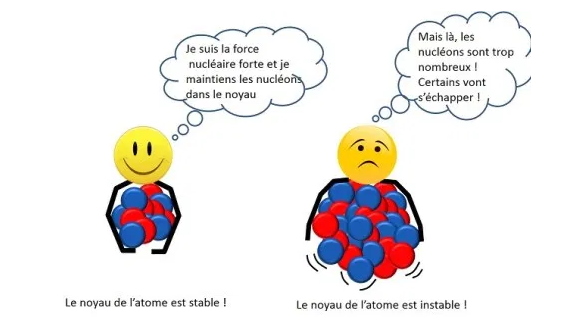
\includegraphics[width=9.597cm,height=5.674cm]{Pictures/10000001000002340000014E5A1981B62E922D6D.png}
\caption{}
\end{figure}

Nucléaire signifie relatif au noyau.

\emph{\textbf{L'énergie nucléaire}} est
l'\href{https://fr.wikipedia.org/wiki/\%C3\%89nergie_(physique)}{\emph{\emph{énergie}}}
associée \emph{\textbf{à la force de cohésion des
}}\href{https://fr.wikipedia.org/wiki/Nucl\%C3\%A9on}{\emph{\emph{\textbf{nucléons}}}}
(\href{https://fr.wikipedia.org/wiki/Proton}{\emph{\emph{protons}}} et
\href{https://fr.wikipedia.org/wiki/Neutron}{\emph{\emph{neutrons}}}),
appelée aussi la
\href{https://fr.wikipedia.org/wiki/Interaction_forte}{\emph{\emph{force
nucléaire forte}}} au sein du noyau des atomes.

\textbf{La radioactivité} est le
\href{https://fr.wikipedia.org/wiki/Ph\%C3\%A9nom\%C3\%A8ne_physique}{\emph{\emph{phénomène
physique}}} par lequel des noyaux atomiques instables se transforment
spontanément en d'autres noyaux (désintégration) en émettant des
particules.

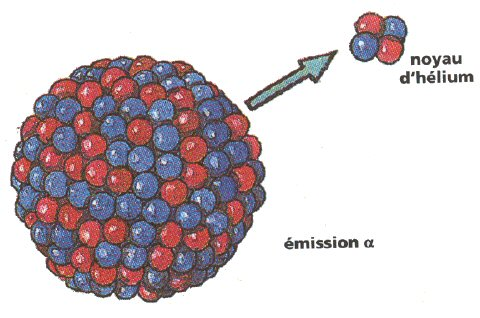
\includegraphics[width=3.117cm,height=2.281cm]{Pictures/10000000000001E00000013EE6B5ED22BED582FE.jpg}Nous
allons envisager dans ce chapitre les réponses à plusieurs questions.

Qu'est ce que la radioactivité ?

D'où provient l'énergie du soleil ?

Pourquoi les réactions nucléaires produisent-elles beaucoup d'énergie ?

Pourquoi les rayonnements radioactifs peuvent-ils être dangereux ?

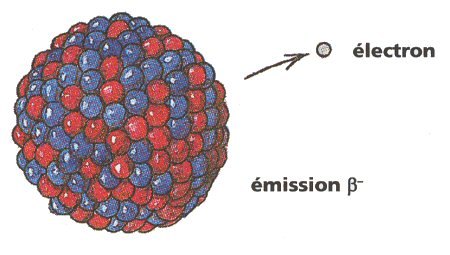
\includegraphics[width=3.353cm,height=2.281cm]{Pictures/10000000000001C2000000FF8E8D24A81F4812A1.jpg}Il
y a-t-il des sources de rayonnements radioactifs naturelles ou
uniquement artificielles ?

Comment fonctionne une centrale nucléaire ?

Quel est le principe de fonctionnement d'une bombe atomique et d'une
bombe H ?

Utilité de la matière radioactive en médecine et en archéologie ?

Que signifie la relation~: E=mc\textsuperscript{2}~?

Que signifie fusion et fission~?

Comment fonctionne la datation au carbone 14~?

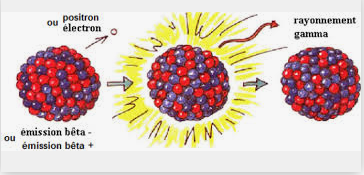
\includegraphics[width=6.421cm,height=3.082cm]{Pictures/100000010000016C000000AF47CF8A96233610D0.png}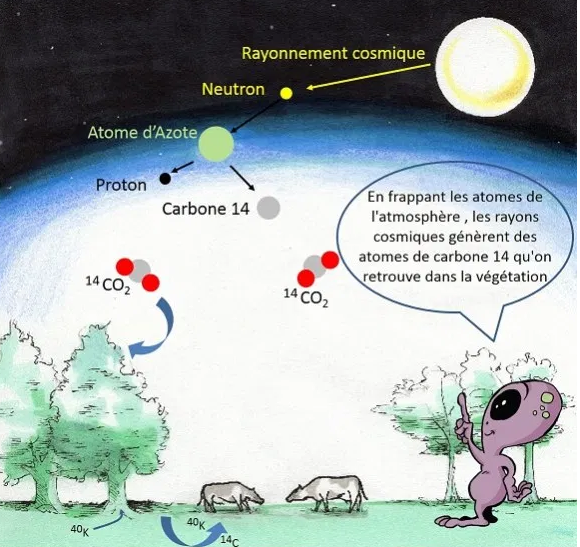
\includegraphics[width=6.144cm,height=5.784cm]{Pictures/1000000100000244000002230722677727C350FD.png}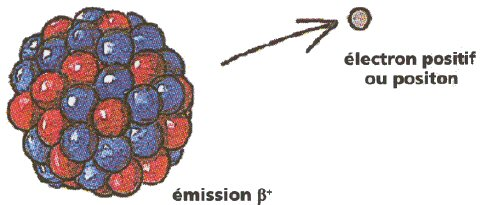
\includegraphics[width=4.105cm,height=1.646cm]{Pictures/10000000000001E0000000CD0A7EA401296A8942.jpg}Qu'est
ce que l'antimatière~?

\begin{figure}
\centering
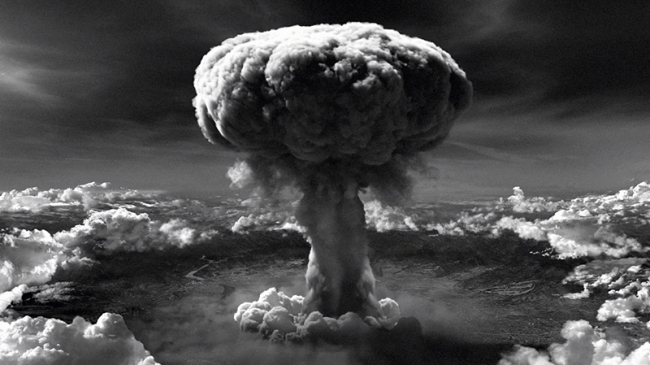
\includegraphics[width=4.35cm,height=2.439cm]{Pictures/100000000000028A0000016D9B2BB1B3B682BBBA.jpg}
\caption{}
\end{figure}

\begin{figure}
\centering
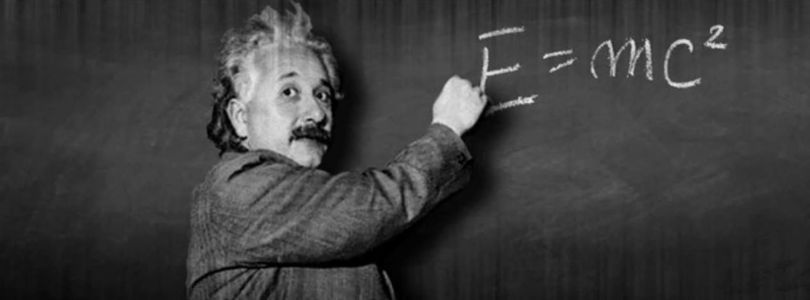
\includegraphics[width=4.942cm,height=1.831cm]{Pictures/100000000000032A0000012C7D9EB773B1A5CFD2.jpg}
\caption{}
\end{figure}

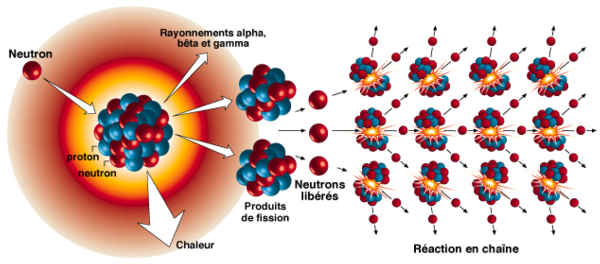
\includegraphics[width=6.451cm,height=2.836cm]{Pictures/1000000000000258000001081538D49477005002.jpg}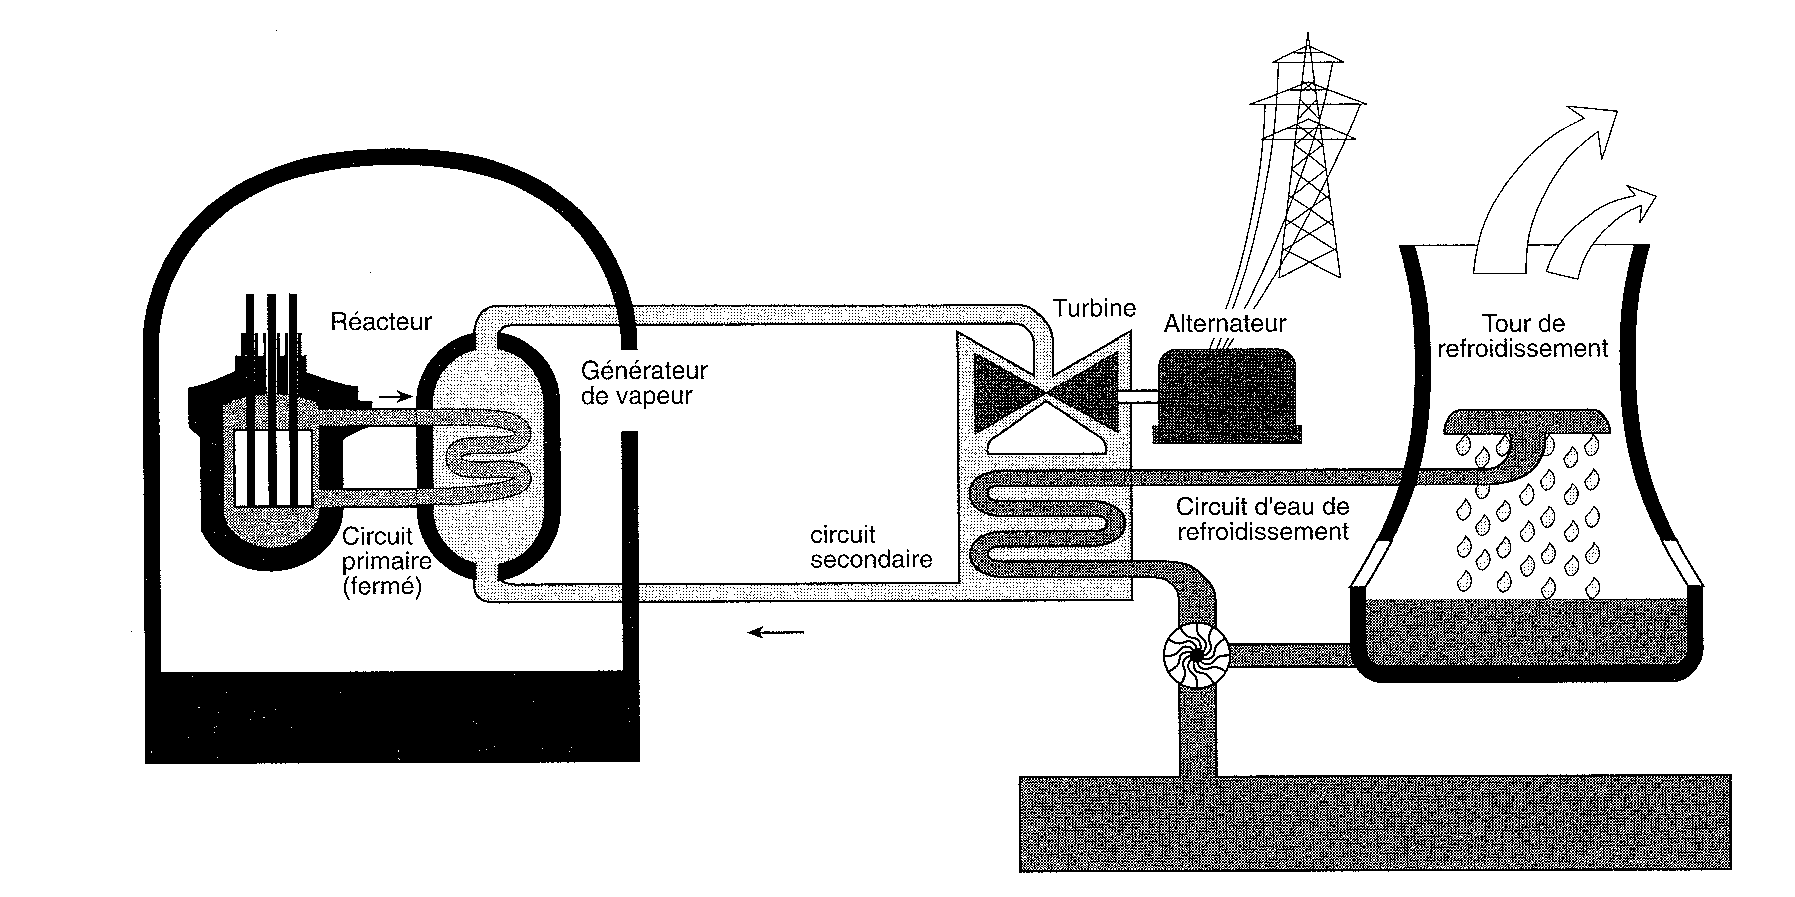
\includegraphics[width=5.801cm,height=2.82cm]{Pictures/1000000000000703000003811303CD635F28D921.png}

\emph{\textbf{1 -- Rappels~:}}

\emph{\textbf{ }}

\begin{enumerate}
\def\labelenumi{\alph{enumi})}
\tightlist
\item
  \emph{la structure du noyau atomique}
\end{enumerate}

Un nucléon est une particule du noyau atomique, donc soit un proton,
soit un neutron.

\begin{figure}
\centering
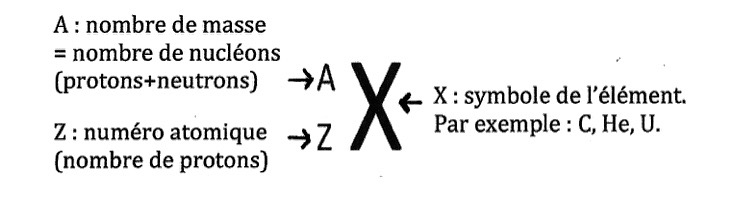
\includegraphics[width=14.063cm,height=3.81cm]{Pictures/10000000000002DD000000C657B445FAE2BE03DE.jpg}
\caption{}
\end{figure}

\begin{enumerate}
\def\labelenumi{\alph{enumi})}
\tightlist
\item
  \emph{Isotopes~: définition. }
\end{enumerate}

Deux isotopes d'un même élément \textbf{se différencient par leur nombre
de neutrons}. Ils possèdent donc le même nombre de protons.

\textbf{Le nombre de neutrons est donc égal à A-Z}

\emph{c) Exemples}~:

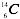
\includegraphics[width=0.706cm,height=0.683cm]{Pictures/1000000100000014000000139893D1A91E50D164.png}
possède 14 nucléons dont 6 protons et 8 neutrons.

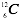
\includegraphics[width=0.706cm,height=0.683cm]{Pictures/100000010000001400000013946388155A247608.png}
est un isotope du
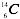
\includegraphics[width=0.706cm,height=0.683cm]{Pictures/1000000100000014000000139893D1A91E50D164.png}.
Il possède 12 nucléons, dont 6 protons et 6 neutrons.

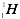
\includegraphics[width=0.706cm,height=0.683cm]{Pictures/100000010000001400000013CF06E53ED3B18878.png}
possède 1 nucléon. C'est un proton.
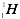
\includegraphics[width=0.706cm,height=0.683cm]{Pictures/100000010000001400000013CF06E53ED3B18878.png}
n'a pas de neutron. Il est appelé le \textbf{protium.}

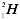
\includegraphics[width=0.706cm,height=0.683cm]{Pictures/1000000100000014000000131B86356A5F025E11.png}est
un isotope de
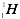
\includegraphics[width=0.706cm,height=0.683cm]{Pictures/100000010000001400000013CF06E53ED3B18878.png}.
Il possède 2 nucléons, dont un proton et un neutron. Il est appelé le
\textbf{deutérium.}

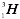
\includegraphics[width=0.706cm,height=0.683cm]{Pictures/100000010000001400000013911DE4B8F4DAD2EC.png}
est un isotope de l'hydrogène. Il possède 3 nucléons, dont 2 neutrons et
1 proton. Il est appelé le \textbf{tritium.}

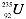
\includegraphics[width=0.918cm,height=0.683cm]{Pictures/100000010000001A000000131DF4E77671AB3F6E.png}
possède 235 nucléons , dont 143 neutrons et 92 protons.

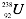
\includegraphics[width=0.918cm,height=0.683cm]{Pictures/100000010000001A000000137145F016F0439DB0.png}possède
238 nucléons, dont 146 neutrons et 92 protons.

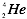
\includegraphics[width=0.966cm,height=0.683cm]{Pictures/100000010000001B00000013CE6DE589828DD379.png}
possède 4 nucléons, dont 2 protons et deux neutrons.

\begin{enumerate}
\def\labelenumi{\alph{enumi})}
\setcounter{enumi}{3}
\tightlist
\item
  \emph{Représentation nucléaire de l'électron, du proton, du neutron et
  du photon}
\end{enumerate}

Des considérations précédentes, il découle~:

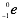
\includegraphics[width=0.683cm,height=0.683cm]{Pictures/100000010000001300000013933991303C233C5E.png}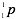
\includegraphics[width=0.613cm,height=0.683cm]{Pictures/10000001000000110000001313D14D1355E58698.png}

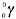
\includegraphics[width=0.565cm,height=0.683cm]{Pictures/10000001000000100000001384CE4DB1D643C8F9.png}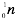
\includegraphics[width=0.565cm,height=0.683cm]{Pictures/10000001000000100000001354D441094A28B79D.png}

\emph{\textbf{2 -- Radioactivité - Trois types de rayonnements
nucléaires. }}

La radioactivité est le
\href{https://fr.wikipedia.org/wiki/Ph\%C3\%A9nom\%C3\%A8ne_physique}{\emph{\emph{phénomène
physique}}} par lequel \textbf{des
}\href{https://fr.wikipedia.org/wiki/Noyau_atomique}{\emph{\emph{\textbf{noyaux
atomiques}}}}\textbf{ instables} (dits radio-nucléides ou
\href{https://fr.wikipedia.org/wiki/Radioisotope}{\emph{\emph{radio-isotopes}}})
\textbf{se transforment }\emph{\textbf{spontanément}} en d'autres atomes
(\href{https://fr.wikipedia.org/wiki/D\%C3\%A9sint\%C3\%A9gration_radioactive}{\emph{\emph{\textbf{désintégration}}}}\textbf{)}
\textbf{en émettant} simultanément \textbf{des particules de matière}
(\href{https://fr.wikipedia.org/wiki/\%C3\%89lectron}{\emph{\emph{électrons}}},
\href{https://fr.wikipedia.org/wiki/Noyau_atomique}{\emph{\emph{noyaux}}}
d'\href{https://fr.wikipedia.org/wiki/H\%C3\%A9lium_4}{\emph{\emph{hélium}}},
\href{https://fr.wikipedia.org/wiki/Neutron}{\emph{\emph{neutrons}}},~etc.)
et /ou des \textbf{photons}.

La radioactivité a été découverte en
\href{https://fr.wikipedia.org/wiki/1896}{\emph{\emph{1896}}} par
\href{https://fr.wikipedia.org/wiki/Henri_Becquerel}{\emph{\emph{Henri
Becquerel}}} dans le cas de
l'\href{https://fr.wikipedia.org/wiki/Uranium}{\emph{\emph{uranium}}},
et très vite confirmée par
\href{https://fr.wikipedia.org/wiki/Marie_Curie}{\emph{\emph{Marie
Curie}}} pour le
\href{https://fr.wikipedia.org/wiki/Radium}{\emph{\emph{radium}}}.
Concernant l'historique (passionnante), je vous propose de lire le livre
pages 188 et 189.

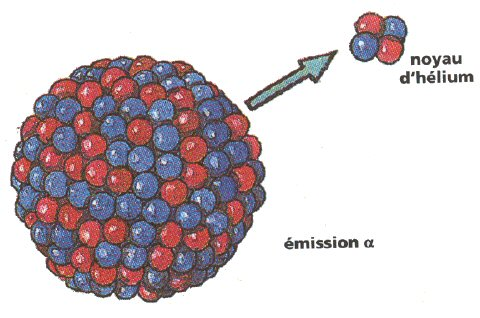
\includegraphics[width=5.697cm,height=3.856cm]{Pictures/10000000000001E00000013EE6B5ED22BED582FE.jpg}\emph{\textbf{2.1.
Il existe trois types de rayonnements nucléaires. }}

\begin{enumerate}
\def\labelenumi{\alph{enumi})}
\tightlist
\item
  \emph{\textbf{Le rayonnement }\textbf{}}~:\textbf{
  }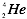
\includegraphics[width=0.966cm,height=0.683cm]{Pictures/100000010000001B00000013CE6DE589828DD379.png}
\end{enumerate}

Un noyau instable se débarrasse d'un groupe de 2 neutrons et deux
protons, autrement dit un noyau d'hélium. Il est appelé \textbf{rayon
.}

\emph{A titre d'exemples~:}

1) L'uranium
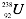
\includegraphics[width=0.918cm,height=0.683cm]{Pictures/100000010000001A000000137145F016F0439DB0.png}se
transmute en thorium lors de sa désintégration en émettant une particule
.

La réaction de désintégration est~:

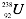
\includegraphics[width=0.918cm,height=0.683cm]{Pictures/100000010000001A000000137145F016F0439DB0.png}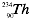
\includegraphics[width=1.059cm,height=0.683cm]{Pictures/100000010000001E000000138E6A8FDDE5499982.png}
+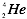
\includegraphics[width=0.966cm,height=0.683cm]{Pictures/100000010000001B00000013CE6DE589828DD379.png}\textbf{
}(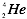
\includegraphics[width=0.966cm,height=0.683cm]{Pictures/100000010000001B00000013CE6DE589828DD379.png}
étant une particule ).

Remarquez que le nombre de protons et neutrons restent constants~:
238=234 +4 et 92=90+2

Pourquoi le Thorium
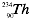
\includegraphics[width=1.059cm,height=0.683cm]{Pictures/100000010000001E000000138E6A8FDDE5499982.png}
? C'est l'élément qui a un numéro atomique Z égal à 90 si vous regardez
dans le tableau périodique de Mendeleïev.

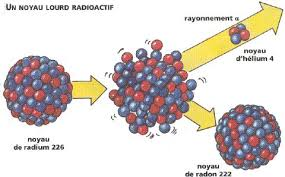
\includegraphics[width=4.75cm,height=2.903cm]{Pictures/100000000000011D000000B18BB391CD0E0D8FA2.jpg}2)
Le radium 226 se transforme en un noyau de radon lors de sa
désintégration et expulse une particule .

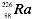
\includegraphics[width=1.177cm,height=0.683cm]{Pictures/100000010000002100000013A43BFC64E9247A2A.png}
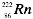
\includegraphics[width=1.177cm,height=0.683cm]{Pictures/100000010000002100000013E5BE5263AA80663E.png}
+
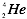
\includegraphics[width=0.966cm,height=0.683cm]{Pictures/100000010000001B00000013CE6DE589828DD379.png}

Lors d'une désintégration, l'élément radioactif se transforme en un
autre élément appelé
\href{https://fr.wikipedia.org/wiki/Produit_de_d\%C3\%A9sint\%C3\%A9gration}{\emph{\emph{produit
de désintégration}}}. Ce produit de désintégration est généralement
lui-même radioactif, et sa propre désintégration conduira à un troisième
élément, et ainsi de suite. Le noyau radioactif atteindra une
configuration stable non radioactive.

Nous illustrerons certaines familles de désintégrations à la fin du
chapitre relatif au trois types de désintégrations.

\begin{figure}
\centering
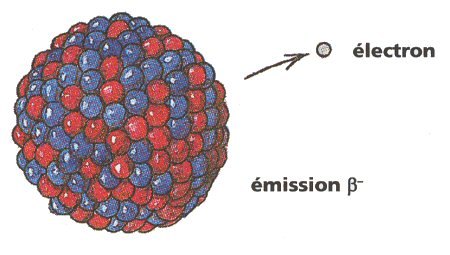
\includegraphics[width=5.373cm,height=3.103cm]{Pictures/10000000000001C2000000FF8E8D24A81F4812A1.jpg}
\caption{}
\end{figure}

\begin{enumerate}
\def\labelenumi{\alph{enumi})}
\tightlist
\item
  \emph{\textbf{Le rayonnement }\textbf{}\textbf{ (électrons ou
  positons) }}
\end{enumerate}

\emph{b.1 -- Le rayonnement }\textsuperscript{\emph{-}}\emph{ (des
électrons~}: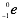
\includegraphics[width=0.683cm,height=0.683cm]{Pictures/100000010000001300000013933991303C233C5E.png}
)\emph{ }

\textbf{Un des neutrons du noyau se transforme en un proton} (c'est
possible en physique quantique) qui reste dans le noyau et \textbf{un
électron est éjecté.}

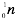
\includegraphics[width=0.565cm,height=0.683cm]{Pictures/10000001000000100000001354D441094A28B79D.png}

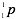
\includegraphics[width=0.613cm,height=0.683cm]{Pictures/10000001000000110000001313D14D1355E58698.png}
+
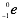
\includegraphics[width=0.683cm,height=0.683cm]{Pictures/100000010000001300000013933991303C233C5E.png}

\emph{Exemple~}: le carbone 14
(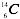
\includegraphics[width=0.706cm,height=0.683cm]{Pictures/1000000100000014000000139893D1A91E50D164.png})
qui sert notamment à la datation au carbone 14 (lisez les pages 193 et
194)

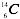
\includegraphics[width=0.706cm,height=0.683cm]{Pictures/1000000100000014000000139893D1A91E50D164.png}

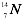
\includegraphics[width=0.825cm,height=0.683cm]{Pictures/10000001000000170000001387F43E8F08B678A8.png}
+
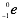
\includegraphics[width=0.683cm,height=0.683cm]{Pictures/100000010000001300000013933991303C233C5E.png}
(remarquez la conservation~: 14 =14 + 0 et 6 = 7 -1)

\emph{b.2 -- Le rayonnement }\textsuperscript{\emph{+}}\emph{ (des
positons(électrons positifs)}
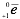
\includegraphics[width=0.706cm,height=0.683cm]{Pictures/1000000100000014000000131B1712312E317641.png}
)

\begin{figure}
\centering
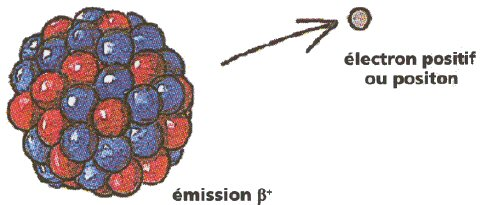
\includegraphics[width=5.373cm,height=2.281cm]{Pictures/10000000000001E0000000CD0A7EA401296A8942.jpg}
\caption{}
\end{figure}

\textbf{Un des protons du noyau se transforme en un neutron}, qui reste
dans le noyau, et un positon est éjecté (un positon est électron positif
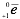
\includegraphics[width=0.706cm,height=0.683cm]{Pictures/1000000100000014000000131B1712312E317641.png}).

\includegraphics[width=0.613cm,height=0.683cm]{Pictures/10000001000000110000001313D14D1355E58698.png}

\includegraphics[width=0.565cm,height=0.683cm]{Pictures/10000001000000100000001354D441094A28B79D.png}
+
\includegraphics[width=0.706cm,height=0.683cm]{Pictures/1000000100000014000000131B1712312E317641.png}

\emph{Exemple~: }

\includegraphics[width=0.683cm,height=0.683cm]{Pictures/10000001000000130000001334A778854DA43436.png}

\includegraphics[width=0.847cm,height=0.683cm]{Pictures/10000001000000180000001378E4F6B83F114C0B.png}
+
\includegraphics[width=0.706cm,height=0.683cm]{Pictures/1000000100000014000000131B1712312E317641.png}

\emph{Remarques~: }

1) Une application médicale est la tomographie par émission de positons
(lire pages 213 et 214)~.

2) Le positon est un exemple d'antimatière. Ce nouveau type de matière,
découverte en 1932, est identique à la matière ordinaire, mais possède
une charge électrique de signe opposé. Il existe donc des antiprotons et
des antineutrons. On a réussi à fabriquer des antiatomes d'hydrogène. La
raison pour actuelle l'Univers actuel est constitué quasi exclusivement
de matière sans antimatière reste, à l'heure actuelle, une des plus
grandes énigmes de la physique.

\begin{figure}
\centering
\includegraphics[width=6.421cm,height=3.082cm]{Pictures/100000010000016C000000AF47CF8A96233610D0.png}
\caption{}
\end{figure}

\begin{enumerate}
\def\labelenumi{\alph{enumi})}
\tightlist
\item
  \emph{\textbf{Le rayonnement }\textbf{}\textbf{ (ondes
  électromagnétiques de très hautes fréquences)~}}\textbf{:
  }\includegraphics[width=0.565cm,height=0.683cm]{Pictures/10000001000000100000001384CE4DB1D643C8F9.png}
\end{enumerate}

La plupart des noyaux provenant d'une désintégration sont produits dans
un état excité, riche en énergie (notation~: X*). Ce \textbf{surplus
d'énergie est libéré }dans les instants qui suivent la désintégration
par l'émission d'un \textbf{rayonnement électromagnétique} de très
grande fréquence. Ce sont les ondes électromagnétiques  de plus hautes
fréquences (et donc de plus grandes énergies~: E = hf) que vous
retrouvez dans le spectre des ondes électromagnétiques.

\emph{Exemple~}:

Un exemple typique est fourni par la désexcitation du
\includegraphics[width=1.177cm,height=0.683cm]{Pictures/100000010000002100000013F4346A116177CC55.png},
lui-même issu de la désintégration \textsuperscript{- }du
\includegraphics[width=1.13cm,height=0.683cm]{Pictures/100000010000002000000013EC637266C7BF3BB2.png}

Une première désintégration \textsuperscript{+~ : }
\includegraphics[width=1.13cm,height=0.683cm]{Pictures/100000010000002000000013EC637266C7BF3BB2.png}

\includegraphics[width=1.177cm,height=0.683cm]{Pictures/100000010000002100000013F4346A116177CC55.png}
+
\includegraphics[width=0.706cm,height=0.683cm]{Pictures/1000000100000014000000131B1712312E317641.png}

Suivie d'une émission
\includegraphics[width=0.354cm,height=0.495cm]{Pictures/100000010000000A0000000EB444449CB8FB105E.png}\textbf{
:
}\includegraphics[width=1.177cm,height=0.683cm]{Pictures/100000010000002100000013F4346A116177CC55.png}
\includegraphics[width=1.177cm,height=0.683cm]{Pictures/100000010000002100000013061F8CC345B56CF4.png}+
\includegraphics[width=0.565cm,height=0.683cm]{Pictures/10000001000000100000001384CE4DB1D643C8F9.png}

\emph{\textbf{Chaine de désintégration de
l'}}\includegraphics[width=0.918cm,height=0.683cm]{Pictures/100000010000001A000000137145F016F0439DB0.png}\textbf{
}\emph{\textbf{- Illustration}}

\begin{figure}
\centering
\includegraphics[width=11.204cm,height=8.608cm]{Pictures/10000001000002E90000023C8DC9DA56C35BDFC0.png}
\caption{}
\end{figure}

\begin{figure}
\centering
\includegraphics[width=11.305cm,height=7.361cm]{Pictures/100000010000022100000163C6AFC1C203E09AFE.png}
\caption{}
\end{figure}

\emph{\textbf{3 -- La décroissance radioactive et activité d'une source
}}

La désintégration radioactive est un phénomène aléatoire : chaque
désintégration est un événement indépendant et l'on ne peut pas prévoir
à quel moment un noyau donné va subir une désintégration.

Par contre, la probabilité qu'il se désintègre endéans un certain laps
de temps est une constante.

Il s'ensuit une loi qui décrit l'évolution au fil du temps du nombre de
noyaux non encore désintégrés.

L'observation montre que la quantité de noyaux instables se trouve
réduite de moitié au bout d'une durée (T~: appelée demi-vie)
caractéristique du noyau considéré.

\begin{figure}
\centering
\includegraphics[width=6.147cm,height=4.33cm]{Pictures/10000001000000DB0000009A3ECA1A1B4D2021A5.png}
\caption{}
\end{figure}

Les demi-vies peuvent avoir des valeurs très diverses,

allant de 10\textsuperscript{-20} secondes à 10\textsuperscript{16
}années.

Quelques exemples ci-contre.

A titre d'exemple, la demi-vie de l'iode 131 est de plus ou moins 8
jours.

Cela signifie~:

- qu'après 8 jours, la moitié de la quantité initiale subsiste,

- qu'après 16 jours, le quart de la quantité initiale subsiste,

- qu'après 24 jours, la huitième de la quantité initiale subsiste,

- qu'après 32 jours, la seizième de la quantité initiale
subsiste,\ldots{}

\begin{figure}
\centering
\includegraphics[width=6.549cm,height=4.221cm]{Pictures/1000000100000179000000F3681E4F513A824012.png}
\caption{}
\end{figure}

\begin{figure}
\centering
\includegraphics[width=1.812cm,height=1.294cm]{Pictures/10000001000000330000002555510415F0E74C8B.png}
\caption{}
\end{figure}

Application~: la datation au carbone 14 (lire le point 4, page 193 et
194).

Activité d'une source (A)

L'activité d'une source radioactive est le nombre de désintégrations par
unité de temps ayant lieu.

Elle est symbolisée par A.

Son unité est le becquerel noté Bq

La radioactivité est un phénomène naturel. Nous sommes baignés dans un
environnement où partout il y a un peu de radioactivité : les aliments,
l'eau, les matériaux de construction de la maison, le rayonnement
cosmiques, certains minéraux terrestres, \textbf{essentiellement le
radon.}

Nous mêmes, nous sommes également faits de quelques éléments radioactifs
en particulier à cause de notre alimentation (surtout à cause de
\textsuperscript{\textbf{40}}K). En moyenne, l'activité du corps humain
est de 8 000 Bq.

\emph{\textbf{4 --} \textbf{Effets biologiques des rayonnements
radioactifs. ( Lire pages 195-196-197)}}

Les particules  et , ainsi que le rayonnement  émis au cours des
réactions nucléaires sont très énergétiques et peuvent, en traversant la
matière, arracher des électrons aux atomes ou rompre des liaisons
chimiques, ce qui aboutit dans la plupart des cas à créer des ions. On
parle \textbf{d'ionisation }de la matière.

La radioactivité est un phénomène naturel. Nous sommes baignés dans un
environnement où partout il y a un peu de radioactivité : les aliments,
l'eau, les matériaux de construction de la maison, le rayonnement
cosmiques, certains minéraux terrestres, essentiellement le radon

Nous mêmes, nous sommes également faits de quelques éléments radioactifs
en particulier à cause de notre alimentation (surtout à cause de
\textsuperscript{\textbf{40}}K). En moyenne, l'activité du corps humain
est de 8 000 Bq.

\emph{\textbf{Caractéristiques des trois types de radiation}}

Les trois types de rayonnement (,  ou ) sont ionisants mais ont des
pouvoirs de pénétration différents dans l'organisme. En effet, leur
parcours se termine lorsque toute l'énergie initiale a été transférée à
la matière qui les arrête.

La longueur de la trajectoire dans un milieu est appelé~: pouvoir de
pénétration.

\begin{figure}
\centering
\includegraphics[width=6.574cm,height=3.461cm]{Pictures/10000001000000DA0000007380CB3B303A836040.png}
\caption{}
\end{figure}

Le danger augmente avec l'activité de la source radioactive, la
proximité de la source, la durée d'exposition et le type de
radioactivité~:

\begin{itemize}
\tightlist
\item
  les particules  sont arrêtées par une feuille de papier ;
\item
  les particules  par une fine plaque d'aluminium ;
\item
  le rayonnement  par une forte épaisseur de plomb ou de béton).
\end{itemize}

\includegraphics[width=4.115cm,height=3.741cm]{Pictures/100000010000018600000162E2F7BB9DEC874BD7.png}\emph{\textbf{La
mesure des doses d'irradiation}}

On parle \textbf{d'irradiation} lorsqu'un organisme se trouve à
proximité d'une source radioactive. Il reçoit alors une partie du
rayonnement émis par la source.

Il y a \textbf{contamination }lorsque les produits radioactifs sont
absorbés par les voies digestives ou respiratoires. Ils peuvent alors se
désintégrer au sein même de l'organisme.

Dans les tissus vivants (voir ci-dessous), les dommages causés par les
rayonnements ne dépendent pas que de l'activité de la source, ils sont
aussi fonction de la nature du rayonnement considéré, et de la nature du
tissu irradié.

Pour évaluer les \textbf{effets physiologiques} des radiations
ionisantes sur l'organisme humain, les doses reçues par le corps humain
se mesurent en \textbf{sieverts (Sv). }

\begin{figure}
\centering
\includegraphics[width=7.28cm,height=5.726cm]{Pictures/100000010000027A000001F28EDBC323318C37DA.png}
\caption{}
\end{figure}

\emph{\textbf{5 -- Forces à l'intérieur du noyau }}

\emph{\textbf{a) Portée et intensité des forces nucléaire et
électrique}} .

Si la force électrique était la seule à l'œuvre dans les noyaux, la
répulsion électrique entre les protons disloquerait immédiatement les
noyaux.

Il faut donc supposer l'existence d'une \textbf{force d'attraction très
intense entre les nucléons. }

\textbf{Cette force, appelée force d'interaction nucléaire forte }(ou
force nucléaire) est une des forces fondamentales de l'Univers, au même
titre que la force de gravitation et la force électrique.

\textbf{La force nucléaire attractive s'exerce entre tous les nucléons,
aussi bien entre proton et proton, qu'entre proton et neutron, qu'entre
neutron et neutron. }

\textbf{Cette force ne s'applique qu'à très courte distance, de l'ordre
de deux à trois fois le diamètre nucléaire (soit
2.10}\textsuperscript{\textbf{-15}}\textbf{ m) et est bien plus intense
que la force électrique sur cette distance. Au-delà de cette distance,
la force électrique (de répulsion entre les protons) prend le dessus. }

\begin{enumerate}
\def\labelenumi{\alph{enumi})}
\setcounter{enumi}{1}
\tightlist
\item
  \emph{\textbf{Ligne de stabilité}}
\end{enumerate}

La force nucléaire ne s'exerce que sur les nucléons proches du noyau, du
fait de sa courte portée.

Dans les petits noyaux (Z  20), un nombre N de neutrons
approximativement égal au nombre Z de protons suffit à stabiliser le
noyau.

Dans les noyaux plus gros, la stabilité est progressivement mise en
péril par l'augmentation du nombre de protons suffisamment éloignés pour
la force électrique prenne petit à petit le dessus sur la force
nucléaire.

Plus un noyau comporte de nucléons, plus il faut que le nombre de
neutrons excède celui des protons pour que l'assemblage reste
\textbf{\textbf{stable}} : c'est ainsi que les noyaux d'atomes présents
dans la nature se situent dans ce qu'on appelle la
\emph{\textbf{«~vallée de stabilité~»}} sur un diagramme comparant le
nombre de protons et le nombre de neutrons des noyaux.

\includegraphics[width=9.37cm,height=6.091cm]{Pictures/1000000100000162000000E5D8F5C376397D35D9.png}-
La figure ci-contre montre où se répartissent les quelques 3000 isotopes
connus.

Parmi eux, la bande centrale, 256 noyaux sont stables et forment la
ligne de stabilité, souvent appelée «~vallée de la stabilité~».

La vallée de la stabilité ne se poursuit pas au-delà du bismuth(Z=83).
Après le bismuth, tous les noyaux sont instables.

\begin{itemize}
\tightlist
\item
  La zone 1~(excès de nucléons) : c'est la zone des noyaux lourds (N et
  Z élevés et donc A grand). Ce sont des noyaux principalement émetteurs
  .
\item
  La zone 2 (excès de neutrons)~: le noyau contient trop de neutrons et
  ceux-ci se transforment en protons qui restent dans le noyau et en
  électrons qui sont expulsés. Ces noyaux sont des émetteurs
  \textsuperscript{-~}.
\item
  La zone 3 (excès de protons)~: le noyau contient trop de protons et
  ceux-ci se transforment en neutrons, qui restent dans le noyau, et en
  positons qui sont expulsés. Ces noyaux sont des émetteurs
  \textsuperscript{+}
\end{itemize}

\emph{\textbf{6 -- Energie de liaison par nucléon d'un noyau et courbe
d'Aston}}

\textbf{L'énergie de liaison est l'énergie qu'il faudrait fournir pour
détruire complètement un noyau. }

Par exemple, c'est l'énergie requise pour séparer un noyau d'hélium
\includegraphics[width=0.966cm,height=0.683cm]{Pictures/100000010000001B00000013CE6DE589828DD379.png}
en 2 protons et 2 neutrons~séparés; ou l'énergie requise pour séparer un
noyau
d'\includegraphics[width=0.918cm,height=0.683cm]{Pictures/100000010000001A000000131DF4E77671AB3F6E.png}
en 143 neutrons et 92 protons séparés.

Ce calcul de l'énergie de liaison nous permet de savoir quel noyau
atomique est le plus stable.

Ce n'est pas tellement la valeur totale de l'énergie de liaison qui
importe. L'uranium a une énergie de liaison phénoménale parce qu'il y a
beaucoup de nucléons à arracher pour détruire le noyau. Ce qui est plus
intéressant, c'est le calcul de la moyenne de l'énergie qu'on doit
fournir à chaque nucléon pour détruire le noyau.

On l'obtient en divisant l'énergie de liaison par le nombre de nucléons
appelée \textbf{énergie de liaison par nucléon (El/nucléon).}

\textbf{Plus l'énergie de liaison par nucléon sera grande, au plus le
noyau sera stable. }

Le graphique (appelé la \emph{\textbf{courbe d'Aston}}) représente
\textbf{l'énergie de liaison par nucléon en fonction du nombre de masse
A}. (Rappel~: A = nombre de protons + nombre de neutrons).

\begin{figure}
\centering
\includegraphics[width=8.348cm,height=6.726cm]{Pictures/1000000000000110000000B9DCC144C0842B84B6.jpg}
\caption{}
\end{figure}

On voit que l'énergie de liaison par nucléon augmente rapidement et
plafonne ensuite à environ 14.10\textsuperscript{-13} J par nucléon.

Elle plafonne, car les nucléons ne sont attirés que par les autres
nucléons voisins. Même si le noyau est plus gros, le nombre de nucléons
voisins reste environ toujours le même et il faut environ
14.10\textsuperscript{-13} J pour arracher un nucléon de ces voisins.

La légère baisse vient de la répulsion électrique qui augmente avec la
grosseur du noyau et qui rend l'extraction des protons plus facile.

On remarque que le noyau qui a le plus d'énergie de liaison par nucléon
est le fer 56 à 14.10\textsuperscript{-13} J/nucléon. C'est dans les
noyaux de fer 56 qu'un nucléon est le plus fermement lié.

\emph{\textbf{Remarque~}}: Utiliser comme unité d'énergie le Joule n'est
pas approprié en énergie nucléaire. Une autre unité d'énergie le plus
souvent utilisée sera l'électron-volt. Cela ne fera pas l'objet de ce
cours mais vous avez l'information.

La valeur de l'électronvolt est définie comme étant
l'\href{https://fr.wikipedia.org/wiki/\%C3\%89nergie_cin\%C3\%A9tique}{\emph{\emph{énergie
cinétique}}} acquise par un
\href{https://fr.wikipedia.org/wiki/\%C3\%89lectron}{\emph{\emph{électron}}}
accéléré depuis le repos par une
\href{https://fr.wikipedia.org/wiki/Potentiel_\%C3\%A9lectrique}{\emph{\emph{différence
de potentiel}}} d'un
\href{https://fr.wikipedia.org/wiki/Volt}{\emph{\emph{volt}}}.

\emph{\textbf{7 -- Le défaut de masse}}

\begin{enumerate}
\def\labelenumi{\alph{enumi})}
\tightlist
\item
  \emph{\textbf{Rappel~: Relation entre unité de masse atomique (uma) et
  kg}}
\end{enumerate}

\textbf{Par définition, une unité de masse atomique (1 uma) correspond à
un douzième de la masse de l'isotope 12 du carbone (dont une mole fait
12 grammes).}

1 mole d'atomes de
\includegraphics[width=0.847cm,height=0.636cm]{Pictures/100000010000001400000013946388155A247608.png}
(soit 6,02.10\textsuperscript{23} atomes) a une masse de 12 g =
12.10\textsuperscript{-3} kg

Donc la masse d'1 atome de
\includegraphics[width=0.706cm,height=0.683cm]{Pictures/100000010000001400000013946388155A247608.png}
=
\includegraphics[width=3.176cm,height=1.177cm]{Pictures/10000001000000A8000000288EBA8C324C0C87D6.png}
kg

Donc 1 uma =
\includegraphics[width=1.694cm,height=0.8cm]{Pictures/100000010000005000000026311100B7BB4DB460.png}=
1,6605.10\textsuperscript{-27} kg

\begin{enumerate}
\def\labelenumi{\alph{enumi})}
\tightlist
\item
  \includegraphics[width=7.375cm,height=4.023cm]{Pictures/100000010000011D0000009C9371CDD98EE4E2B1.png}\emph{\textbf{Le
  défaut de masse }}
\end{enumerate}

Par des techniques très précises, il est possible de mesurer la masse
d'un noyau et celle d'un proton isolé ou d'un neutron isolé. Il s'avère,
découverte surprenante, que \textbf{la masse d'un noyau est inférieure à
la somme des masses de chacun de ses nucléons. ~}

\textbf{Cette différence est appelée l}\emph{\textbf{e défaut de
masse}}\textbf{ m}

\emph{\textbf{Conclusion~:}}

\emph{\textbf{Lors de la formation d'un noyau à partir de protons et
neutrons, il y a diminution de masse.}}

\emph{\textbf{Lors de désintégration d'un noyau en ses différents
nucléons séparés, il y a augmentation de masse. }}

\begin{enumerate}
\def\labelenumi{\alph{enumi})}
\tightlist
\item
  \emph{\textbf{Equivalence masse-énergie}}
\end{enumerate}

Mais où est passée cette masse?

\textbf{En 1905, Einstein établit qu'elle s'est transformée en énergie.}
Dans certaines circonstances, une masse m peut se transformer en énergie
E.

\textbf{Cette quantité d'énergie est l'énergie de liaison et elle
correspond à l'énergie qu'il faut fournir au noyau pour qu'il soit
dissocié en nucléons isolés.}

Il établit la relation d'équivalence~entre la masse et l'énergie.

\emph{\textbf{8 -- Réactions nucléaires et dégagement d'énergie. }}

\textbf{L'équivalence masse-énergie
(E=mc}\textsuperscript{\textbf{2}}\textbf{)} \textbf{est la clé }pour
comprendre le défaut de masse constaté dans les atomes.

\textbf{En effet, le défaut de masse d'un noyau est équivalent à
l'énergie de liaison E}\textsubscript{\textbf{L}}\textbf{ du noyau. }

\emph{\textbf{Les noyaux dans lesquels les nucléons sont moyennement
liés (E}}\textsubscript{\emph{\textbf{l}}}\emph{\textbf{/nucléon
moyenne) qui se transforment en d'autres noyaux au sein desquels
l'énergie de liaison par nucléon est plus importante
(E}}\textsubscript{\emph{\textbf{l}}}\emph{\textbf{/nucléon plus
importante) donneront lieu à une libération d'énergie. }}

\begin{figure}
\centering
\includegraphics[width=7.056cm,height=5.644cm]{Pictures/10000001000000E2000000B4942537CB26E0723C.png}
\caption{}
\end{figure}

La forme de la courbe de stabilité des noyaux permet de prédire que deux
types de réactions nucléaires seront exothermiques.

\begin{itemize}
\tightlist
\item
  D'une part, des réactions qui brisent des noyaux très lourds en
  plusieurs noyaux de masses moyennes et d'énergie par nucléon de
  liaison plus grandes. C'est \emph{\textbf{la fission nucléaire.}}
  C'est\emph{\textbf{ }}l'énergie utilisée dans les \textbf{centrales
  nucléaires.}
\item
  D'autre part, des réactions qui assemblent des noyaux très légers pour
  former un noyau de masse intermédiaire d'énergie de liaison par
  nucléon plus importante. . C'est \emph{\textbf{la fusion nucléaire.}}
  C'est l'énergie utilisée par \textbf{notre Soleil.}
\end{itemize}

\begin{figure}
\centering
\includegraphics[width=5.131cm,height=4.584cm]{Pictures/100000010000013B00000106ADCB5679C9DC9F10.gif}
\caption{}
\end{figure}

\emph{\textbf{a) La réaction de fission nucléaire}}

\includegraphics[width=1.011cm,height=0.728cm]{./ObjectReplacements/Object 1}Lors
de cette réaction nucléaire, un noyau, soumis à l'impact d'un neutron,
se divise en deux.

\includegraphics[width=0.917cm,height=0.683cm]{./ObjectReplacements/Object 2}Un
exemple de réaction de fission est la suivante~:

\includegraphics[width=0.564cm,height=0.683cm]{./ObjectReplacements/Object 3}\includegraphics[width=1.035cm,height=0.635cm]{./ObjectReplacements/Object 8}

\begin{enumerate}
\def\labelenumi{\arabic{enumi})}
\tightlist
\item
  Une énergie (notons la E1) est fournie pour séparer les nucléons du
  noyau de
  l'\includegraphics[width=0.917cm,height=0.683cm]{./ObjectReplacements/Object 9}.
\item
  Une énergie (notons la E2) est libérée pour former les noyaux de
  \includegraphics[width=1.011cm,height=0.728cm]{./ObjectReplacements/Object 10}
  et de
  \includegraphics[width=1.035cm,height=0.635cm]{./ObjectReplacements/Object 11}
  .
\item
  Comme les énergies de liaison par nucléon du
  \includegraphics[width=1.011cm,height=0.728cm]{./ObjectReplacements/Object 12}
  et du
  \includegraphics[width=1.035cm,height=0.635cm]{./ObjectReplacements/Object 13}
  sont supérieures à celle de l'
  \includegraphics[width=0.917cm,height=0.683cm]{./ObjectReplacements/Object 14}
  (voir la courbe d'Aston ci-dessus), le bilan de la réaction libère de
  l'énergie.
\end{enumerate}

\protect\hypertarget{anchor}{}{}

Lors d'une réaction de fission, un noyau lourd, au sein duquel les
nucléons sont moins fortement liés, se transforme en noyaux plus légers,
au sein desquels les nucléons sont plus fortement liés (cf. courbe
d'Aston). Or une énergie de liaison par nucléon plus grande conduit à un
défaut de masse plus important.

Dans le cas de la fission, cette perte de masse résulte de ce que la
dissociation des très gros noyaux permet de constituer des noyaux moins
gros, qui ont une cohésion plus forte puisqu'ils sont caractérisés par
une énergie de liaison par nucléon plus grande, et donc par un défaut de
masse par nucléon plus important. Le même nombre de nucléons se
recombine ainsi en un ensemble atomique de masse moins grande.

\textbf{Il y a diminution de masse, et donc d'énergie. La réaction est
exothermique}

La fission de 1 gramme d'uranium libère une énergie équivalente à
l'énergie chimique contenue dans 2300 litres de mazout~!!!

\begin{enumerate}
\def\labelenumi{\alph{enumi})}
\tightlist
\item
  \emph{\textbf{La réaction de fusion~: énergie du soleil et des
  étoiles.}}
\end{enumerate}

\includegraphics[width=6.683cm,height=3.997cm]{Pictures/10000000000002BC000001A3F2B1BDBB4F71DAC0.jpg}La
réaction nucléaire de fusion est une réaction qui, \textbf{au départ de
petits noyaux,} \textbf{forme un plus gros noyau.}

Un exemple de réaction est la suivante, la fusion du deutérium et du
tritium, isotopes de l'hydrogène.

\begin{figure}
\centering
\includegraphics[width=0.658cm,height=0.635cm]{./ObjectReplacements/Object 15}
\caption{ +
\includegraphics[width=0.658cm,height=0.635cm]{./ObjectReplacements/Object 16}

\includegraphics[width=0.894cm,height=0.635cm]{./ObjectReplacements/Object 17}
+
\includegraphics[width=0.542cm,height=0.635cm]{./ObjectReplacements/Object 18}}
\end{figure}

\begin{figure}
\centering
\includegraphics[width=5.385cm,height=4.209cm]{Pictures/10000000000001DC00000174806216890CE122F5.jpg}
\caption{}
\end{figure}

Lors d'une réaction de fusion, l'énergie nucléaire se dégage car la
masse du noyau obtenu est inférieure à la masse des noyaux initiaux.

Dans le cas de la fusion, cette perte de masse résulte de ce que la
fusion de noyaux légers permet de constituer des atomes plus gros, qui
ont une cohésion plus forte puisqu'ils sont caractérisés par une énergie
de liaison par nucléon plus grande, et donc par un défaut de masse par
nucléon plus important. Le même nombre de nucléons se recombine ainsi en
un ensemble atomique de masse moins grande.

\textbf{Il y a diminution de masse, et donc d'énergie. La réaction est
exothermique.}

\emph{\textbf{Mais pourquoi ne produit-on pas d'énergie en utilisant la
fusion nucléaire au niveau industriel~?}}

Maîtriser sur Terre la fusion de noyaux légers, tels que le
\href{https://fr.wikipedia.org/wiki/Deut\%C3\%A9rium}{\emph{\emph{deutérium}}}
et le tritium donnerait accès à des ressources énergétiques dans des
quantités jamais rencontrées jusqu'alors par l'espèce humaine et
produirait beaucoup moins de déchets nucléaires que la fission.

Si la
\href{https://fr.wikipedia.org/wiki/Fission_nucl\%C3\%A9aire}{\emph{\emph{fission
nucléaire}}} est contrôlée depuis longtemps pour la
\href{https://fr.wikipedia.org/wiki/Production_d\%27\%C3\%A9lectricit\%C3\%A9}{\emph{\emph{production
d'électricité}}} (au niveau des centrales nucléaires), ce n'est pas le
cas de la fusion.

La réaction de fusion nucléaire est une réaction est difficile à
réaliser car il faut rapprocher deux noyaux qui ont tendance
naturellement à se repousser à cause de la force électrique. Il faut
donc parvenir à vaincre la répulsion électrique afin de rapprocher les
noyaux dans le champ de la force nucléaire.

Les énergies nécessaires à la fusion restent très élevées, correspondant
à des
\href{https://fr.wikipedia.org/wiki/Temp\%C3\%A9rature}{\emph{\emph{températures}}}
de plusieurs dizaines ou même centaines de millions de
\href{https://fr.wikipedia.org/wiki/Degr\%C3\%A9_Celsius}{\emph{\emph{degrés
Celsius}}} selon la nature des noyaux. \textbf{Au sein du
}\href{https://fr.wikipedia.org/wiki/Soleil}{\emph{\emph{\textbf{Soleil}}}}\textbf{,
par exemple, la fusion de
l'}\href{https://fr.wikipedia.org/wiki/Hydrog\%C3\%A8ne}{\emph{\emph{\textbf{hydrogène}}}}\textbf{,
qui aboutit par étapes à produire de
l'}\href{https://fr.wikipedia.org/wiki/H\%C3\%A9lium}{\emph{\emph{\textbf{hélium}}}}\textbf{,
s'effectue à des températures de l'ordre de quinze millions de
}\href{https://fr.wikipedia.org/wiki/Kelvin}{\emph{\emph{\textbf{kelvins}}}}\textbf{.
}

\emph{\emph{La fusion est une énergie propre}.\emph{ Elle n'émet pas de
gaz à effet de serre ni de déchets radioactifs à demi-vie
longu}}e\emph{.}

Cet enjeu considérable a mené les communautés scientifiques nationales
et internationales à lancer plusieurs projets d'envergure.

\emph{\textbf{ITER}}~: projet international (35 pays) qui s'inscrit dans
une démarche à long terme visant à l'industrialisation de la fusion
nucléaire. Pourrait-on rêver de la production d'énergie à l'horizon
2035~?

Dans la bombe H (H comme hydrogène), la réaction est possible grâce à
une haute température obtenue, elle-même, par réaction de fission
nucléaire\ldots..

\emph{\textbf{9 -- Application~: la centrale nucléaire}}

\begin{enumerate}
\def\labelenumi{\alph{enumi})}
\tightlist
\item
  \emph{Fonctionnement}
\end{enumerate}

La centrale nucléaire utilisant l'énergie nucléaire n'est rien d'autre
qu'une machine thermique dont la source chaude est un réacteur
nucléaire.

\begin{figure}
\centering
\includegraphics[width=15.898cm,height=7.479cm]{Pictures/10000001000001C3000000D48AB61C0B764D908D.png}
\caption{}
\end{figure}

\hypertarget{le-circuit-primaire}{%
\subsubsection{\texorpdfstring{\emph{\textbf{1. Le circuit
primaire}}}{1. Le circuit primaire}}\label{le-circuit-primaire}}

Dans le \textbf{réacteur (1)}, la fission des atomes d'uranium produit
\textbf{une grande quantité de chaleur}.\\
Cette chaleur fait augmenter \textbf{la température de l'eau} qui
circule autour du réacteur, à 320 °C. L'eau est maintenue sous pression
pour l'empêcher de bouillir. Ce circuit fermé est appelé \textbf{circuit
primaire}.

\hypertarget{le-circuit-secondaire}{%
\subsubsection{\texorpdfstring{\emph{\textbf{2. Le circuit
secondaire}}}{2. Le circuit secondaire}}\label{le-circuit-secondaire}}

Le circuit primaire communique avec un deuxième circuit fermé, appelé
\textbf{circuit secondaire} par l'intermédiaire d'un \textbf{générateur
de vapeur (2)}. Dans ce générateur de vapeur, l'eau chaude du circuit
primaire chauffe l'eau du circuit secondaire qui se transforme en
\textbf{vapeur}. La pression de cette vapeur fait tourner une
\textbf{turbine (3)} qui entraîne à son tour un \textbf{alternateur}.
Grâce à l'énergie fournie par la turbine, \textbf{l'alternateur} produit
\textbf{un courant électrique alternatif.}

\textbf{Un transformateur} élève la tension du courant électrique
produit par l'alternateur pour qu'il puisse être plus facilement
\textbf{transporté dans les lignes très haute tension.}

\hypertarget{le-circuit-de-refroidissement}{%
\subsubsection{\texorpdfstring{\emph{\textbf{3. Le circuit de
refroidissement}}}{3. Le circuit de refroidissement}}\label{le-circuit-de-refroidissement}}

À la sortie de la turbine, la vapeur du circuit secondaire est à nouveau
\textbf{transformée en eau} grâce à un condenseur dans lequel circule de
l'eau froide en provenance de la mer ou d'un fleuve. Ce troisième
circuit est appelé \textbf{circuit de refroidissement (4).}\\
En bord de rivière, l'eau de ce 3\textsuperscript{e} circuit peut alors
être refroidie au contact de l'air circulant dans de grandes tours.

Le grand intérêt des centrales nucléaires est de fournir beaucoup
d'énergie en consommant peu de combustible et en ne rejetant pas de CO2
dans l'atmosphère.

L'utilisation d'un combustible radioactif et non renouvelable et le
stockage des déchets reste un problème non résolu.

\begin{enumerate}
\def\labelenumi{\alph{enumi})}
\tightlist
\item
  \includegraphics[width=7.925cm,height=6.421cm]{Pictures/1000000100000234000001C99805E06609697748.png}\emph{\textbf{Réaction
  en chaine. }}
\end{enumerate}

Dans le domaine du
\href{https://fr.wikipedia.org/wiki/Nucl\%C3\%A9aire}{\emph{\emph{nucléaire}}},
une \textbf{réaction en chaîne} se produit lorsqu'un
\href{https://fr.wikipedia.org/wiki/Neutron}{\emph{\emph{neutron}}}
cause la
\href{https://fr.wikipedia.org/wiki/Fission}{\emph{\emph{fission}}} d'un
noyau
\href{https://fr.wikipedia.org/wiki/Fissile}{\emph{\emph{fissile}}}
produisant un plus grand nombre de neutrons qui à leur tour causent
d'autres fissions.

En effet, un des neutrons, libéré lors de la première fission, rencontre
un autre noyau d'uranium et provoque une nouvelle fission. A son tour,
cette réaction libère des neutrons qui vont atteindre d'autres noyaux
d'uranium situés à proximité amorçant d'autres fissions et ainsi de
suite ..

Une réaction en chaîne non contrôlée, qui se produit avec une quantité
suffisamment importante de
\href{https://fr.wikipedia.org/wiki/Combustible_nucl\%C3\%A9aire}{\emph{\emph{combustible
fissile}}}
(\href{https://fr.wikipedia.org/wiki/Masse_critique_(r\%C3\%A9action_nucl\%C3\%A9aire)}{\emph{\emph{masse
critique}}}) peut mener à une
\href{https://fr.wikipedia.org/wiki/Explosion}{\emph{\emph{explosion}}}
d'\href{https://fr.wikipedia.org/wiki/\%C3\%89nergie}{\emph{\emph{énergie}}},
c'est le principe d'une
\href{https://fr.wikipedia.org/wiki/Bombe_A}{\emph{\emph{bombe
atomique}}}.

\begin{enumerate}
\def\labelenumi{\alph{enumi})}
\tightlist
\item
  \emph{\textbf{Contrôle de la réaction en chaîne dans une centrale
  nucléaire.}}
\end{enumerate}

\includegraphics[width=8.327cm,height=5.385cm]{Pictures/10000001000000DA0000009916BD0968417286CD.png}Dans
une centrale nucléaire, la réaction en chaîne est contrôlée et utilisée
dans un
\href{https://fr.wikipedia.org/wiki/R\%C3\%A9acteur_nucl\%C3\%A9aire}{\emph{\emph{réacteur
nucléaire}}} pour produire de l'énergie.

Lorsqu'un réacteur fonctionne en régime stationnaire, la réaction en
chaine est contrôlée. Plus précisément, sur les 3 neutrons produits par
la réaction de fission, 2 seront capturés par des barres de contrôle.
Ces barres de contrôle sont des barres de cadmium, métal qui a la
propriété d'absorber les neutrons qui l'atteignent. Lorsque toutes les
barres de contrôle d'un réacteur sont abaissées, la réaction en chaine
s'arrête.

L'argumentation concernant l'utilisation des centrales nucléaires ne
sera pas traitée ici. Il s'agit d'un sujet complexe mais vous avez
toutes les informations scientifiques nécessaires à présent pour vous
comporter en citoyen averti et développer votre sens critique en vous
renseignant et documentant afin de vous forger un avis critique.

\emph{\textbf{Lire pages 207 à 214. }}

\emph{\textbf{Exercice 1}}

Ecrire les réactions nucléaires suivantes :

\begin{enumerate}
\def\labelenumi{\alph{enumi})}
\tightlist
\item
  La désintégration  du
  \includegraphics[width=1.177cm,height=0.683cm]{./ObjectReplacements/Object 19}
\end{enumerate}

\begin{enumerate}
\def\labelenumi{\alph{enumi})}
\tightlist
\item
  La désintégration \textsuperscript{-} du
  \includegraphics[width=0.706cm,height=0.683cm]{./ObjectReplacements/Object 20}
\end{enumerate}

\begin{enumerate}
\def\labelenumi{\alph{enumi})}
\tightlist
\item
  La désintégration \textsuperscript{+} du
  \includegraphics[width=0.683cm,height=0.683cm]{./ObjectReplacements/Object 21}
\end{enumerate}

\begin{enumerate}
\def\labelenumi{\alph{enumi})}
\tightlist
\item
  L'émission  du
  \includegraphics[width=1.035cm,height=0.683cm]{./ObjectReplacements/Object 22}*
\end{enumerate}

\emph{\textbf{Exercice 2}}

\begin{enumerate}
\def\labelenumi{\alph{enumi})}
\tightlist
\item
  Combien de demi-vies doivent s'écouler pour que l'activité d'un
  élément décroisse d'un facteur 256?
\end{enumerate}

(Rép : 8 demi-vies)

\begin{enumerate}
\def\labelenumi{\alph{enumi})}
\tightlist
\item
  Après 24 h, la radioactivité d'un élément tombe à 1/8 de sa valeur
  initiale. Que vaut sa demi-vie?
\end{enumerate}

(Rép : 8 h)

\begin{enumerate}
\def\labelenumi{\alph{enumi})}
\tightlist
\item
  L'activité d'un matériau contenant du
  \includegraphics[width=0.706cm,height=0.683cm]{./ObjectReplacements/Object 23}
  est réduite d'un facteur 6. Sachant que la demi-vie du
  \includegraphics[width=0.706cm,height=0.683cm]{./ObjectReplacements/Object 24}
  est de 5730 ans, combien de temps s'est il écoulé depuis la création
  de ce matériau?
\end{enumerate}

(Rép : 14783 ans)

\emph{\textbf{Exercice 3}}

On injecte 1 g
d'\includegraphics[width=0.683cm,height=0.753cm]{./ObjectReplacements/Object 25}
à un patient au cours d'une analyse médicale (scintigraphie). Après
combien de temps n'y aura-t-il plus que 1\% de la dose initiale dans
l'organisme si la demi-vie de
l'\includegraphics[width=0.683cm,height=0.753cm]{./ObjectReplacements/Object 26}
est de 8 jours?

(Rép :53 jours)

\emph{\textbf{Exercice 4}}

\begin{enumerate}
\def\labelenumi{\alph{enumi})}
\tightlist
\item
  Sachant que le soleil rayonne à chaque seconde une énergie de
  7.10\textsuperscript{26} J, calcule la perte de masse de cette étoile
  par seconde. (Rép : 7,8.10\textsuperscript{9} kg)
\end{enumerate}

\begin{enumerate}
\def\labelenumi{\alph{enumi})}
\tightlist
\item
  En supposant que ce processus soit le seul et qu'il ait lieu de la
  même façon jusqu'à la disparition complète de l'astre, calcule le
  temps de vie théorique du soleil.
\end{enumerate}

La masse du soleil est de 2.10\textsuperscript{30} kg. (Rép :
8,2.10\textsuperscript{12} années)

\emph{\textbf{Exercice 5}}

Calculer l'énergie de liaison d'un atome d'hélium
\includegraphics[width=0.965cm,height=0.683cm]{./ObjectReplacements/Object 27}
sachant que sa masse mesurée expérimentalement est de 4,00260 uma.

(Rép : 1,13 pJ)

\emph{\textbf{Exercice 6 (n° 21 page 216)}}

\begin{enumerate}
\def\labelenumi{\alph{enumi})}
\tightlist
\item
  Calculer le défaut de masse du néon 22 sachant que sa masse isotopique
  est de 21,99138 uma.
\end{enumerate}

(Rép : 0,31689.10\textsuperscript{-27} kg)

\begin{enumerate}
\def\labelenumi{\alph{enumi})}
\tightlist
\item
  Calculer son énergie de liaison par nucléon.
\end{enumerate}

(Rép : 1,3 pJ)

\emph{\textbf{Exercice 7( page 206)}}

Calculer l'énergie libérée lors de la désintégration radioactive  de 1
mole de
\includegraphics[width=1.177cm,height=0.683cm]{./ObjectReplacements/Object 28},
sachant que la masse mesurée des atomes est :

m\includegraphics[width=1.177cm,height=0.683cm]{./ObjectReplacements/Object 29}
= 226,02541 uma

m\includegraphics[width=1.177cm,height=0.683cm]{./ObjectReplacements/Object 30}
= 222,01758 uma

m
\includegraphics[width=0.988cm,height=0.683cm]{./ObjectReplacements/Object 31}
= 4,00260 uma

(Rép : 4,7.10\textsuperscript{11} J)

\emph{\textbf{Exercice 8 ( page 204)}}

Calculer la variation d'énergie produite lors de la réaction nucléaire
de fission de 1 gramme d'uranium sachant que l'énergie de liaison par
nucléon des isotopes suivants est :

El/nucléon
\includegraphics[width=0.917cm,height=0.683cm]{./ObjectReplacements/Object 32}
= 1,40 pJ

El/nucléon
\includegraphics[width=1.106cm,height=0.683cm]{./ObjectReplacements/Object 33}
= 1,35 pJ

El/nucléon
\includegraphics[width=0.917cm,height=0.683cm]{./ObjectReplacements/Object 34}
= 1,22 pJ

(Rép : 8,2.10\textsuperscript{10}J)

\emph{\textbf{Exercice 9 (page 205)}}

Calculer la variation d'énergie produite lors de la réaction nucléaire
de fusion de 1 gramme de deutérium-tritium sachant que l'énergie de
liaison par nucléon des isotopes suivants est :

El/ nucléon
\includegraphics[width=0.706cm,height=0.683cm]{./ObjectReplacements/Object 35}
= 0,178 pJ

El/nucléon
\includegraphics[width=0.706cm,height=0.683cm]{./ObjectReplacements/Object 36}
= 0,453 pJ

El/nucléon
\includegraphics[width=0.965cm,height=0.683cm]{./ObjectReplacements/Object 37}
= 1,133 pJ

(Rép : 3,4.10\textsuperscript{11} J)

\includegraphics[width=19.473cm,height=26.859cm]{Pictures/1000000100000262000003488C6E86B2411A3EA3.png}

\includegraphics[width=19.731cm,height=27.236cm]{Pictures/10000001000002620000034931F21BAF71411AAA.png}
